

\tikzset{every picture/.style={line width=0.75pt}} %set default line width to 0.75pt        

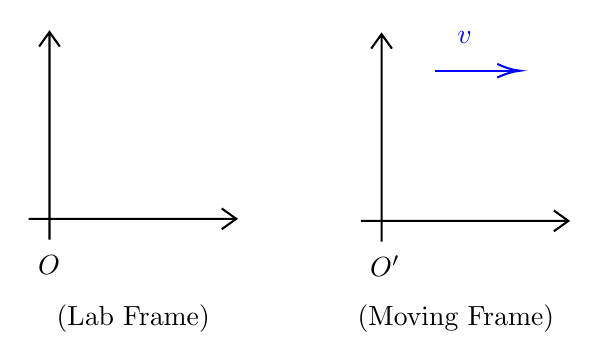
\begin{tikzpicture}[x=0.75pt,y=0.75pt,yscale=-1,xscale=1]
%uncomment if require: \path (0,193); %set diagram left start at 0, and has height of 193

%Shape: Axis 2D [id:dp9794610670096641] 
\draw  (171,118) -- (271,118)(181,28) -- (181,128) (264,113) -- (271,118) -- (264,123) (176,35) -- (181,28) -- (186,35)  ;
%Shape: Axis 2D [id:dp21159834766612584] 
\draw  (331,119) -- (431,119)(341,29) -- (341,129) (424,114) -- (431,119) -- (424,124) (336,36) -- (341,29) -- (346,36)  ;
%Straight Lines [id:da5217345963407499] 
\draw [color={rgb, 255:red, 0; green, 6; blue, 255 }  ,draw opacity=1 ]   (366.68,46.65) -- (405.68,46.65) ;
\draw [shift={(407.68,46.65)}, rotate = 180] [color={rgb, 255:red, 0; green, 6; blue, 255 }  ,draw opacity=1 ][line width=0.75]    (10.93,-3.29) .. controls (6.95,-1.4) and (3.31,-0.3) .. (0,0) .. controls (3.31,0.3) and (6.95,1.4) .. (10.93,3.29)   ;

% Text Node
\draw (376,26.4) node [anchor=north west][inner sep=0.75pt]  [color={rgb, 255:red, 0; green, 6; blue, 255 }  ,opacity=1 ]  {$v$};
% Text Node
\draw (174,134.4) node [anchor=north west][inner sep=0.75pt]    {$O$};
% Text Node
\draw (334,134.4) node [anchor=north west][inner sep=0.75pt]    {$O'$};
% Text Node
\draw (183,158) node [anchor=north west][inner sep=0.75pt]   [align=left] {(Lab Frame)};
% Text Node
\draw (328,158) node [anchor=north west][inner sep=0.75pt]   [align=left] {(Moving Frame)};


\end{tikzpicture}
